 
\section{Aufgabe 1: \emph{Polynom}}

\begin{figure}
\centering
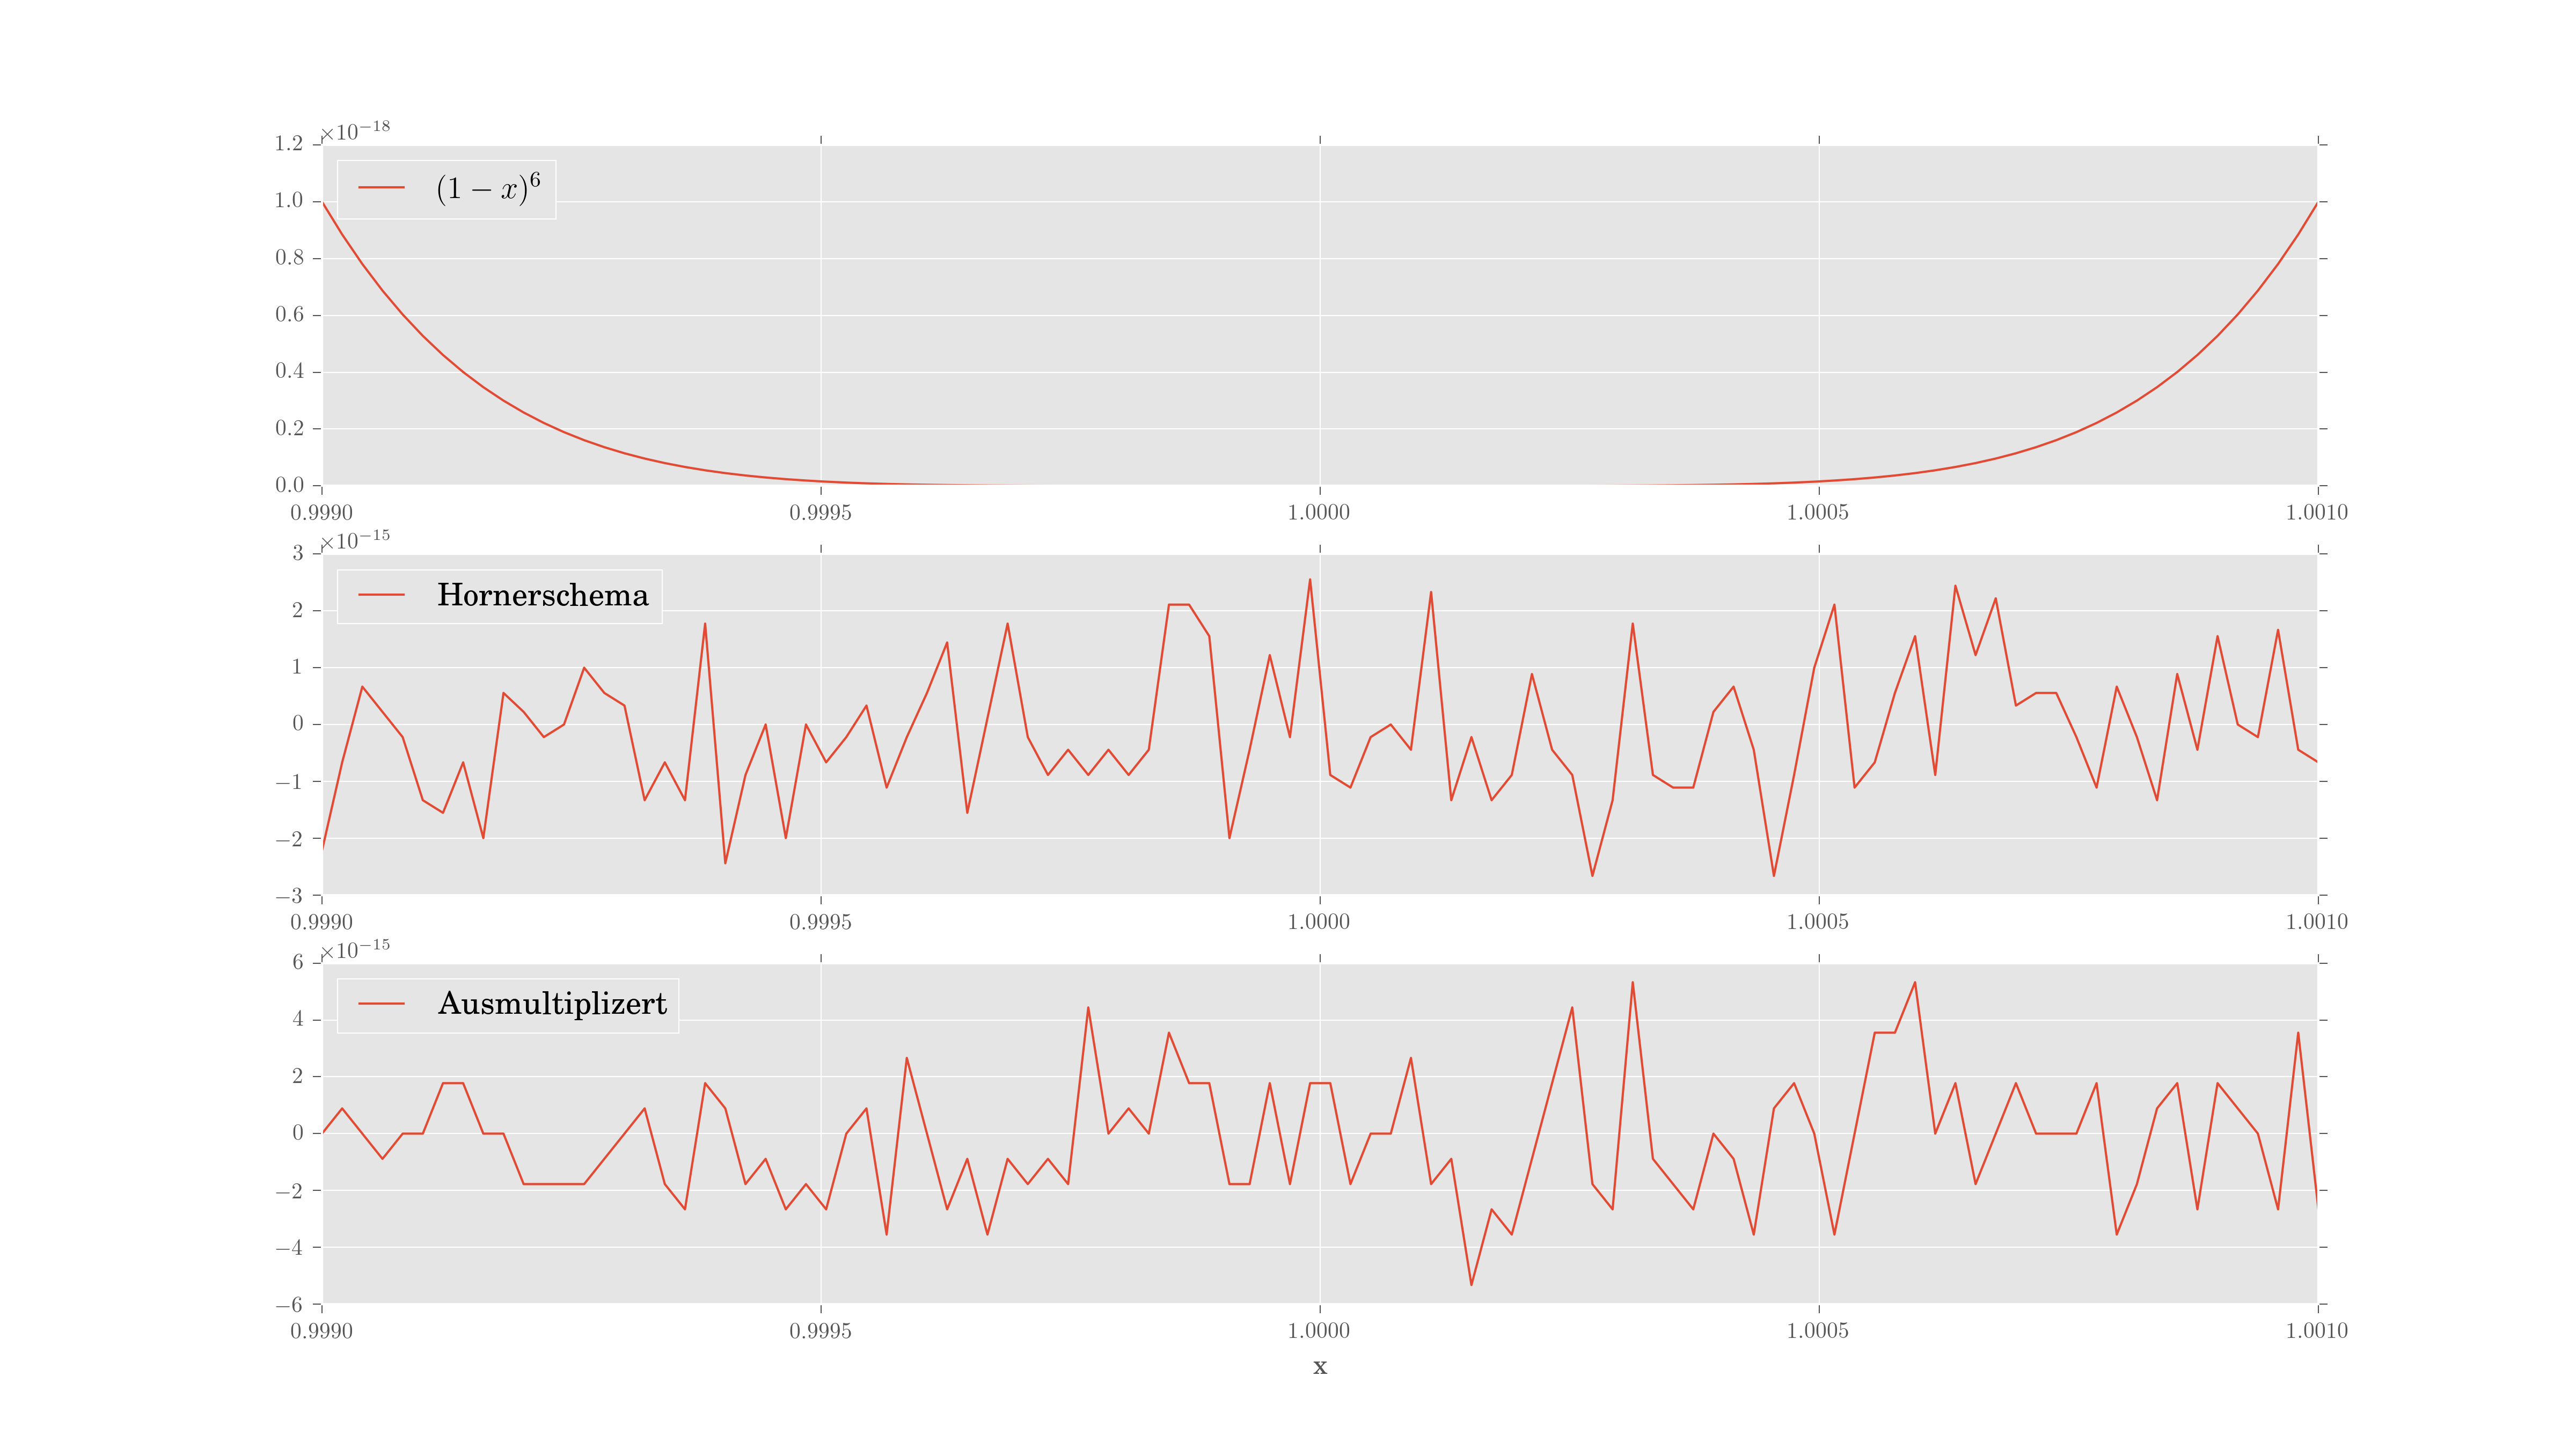
\includegraphics[width=\textwidth]{plot1.png}
\caption{Auswertung des Polynoms $f(x)=(1-x)⁶$. Es wird direkt, durch ausmultiplizieren auf naive Weise und mit dem Horner-Schema berechnet.}
\end{figure}

\section{Aufgabe 2: \emph{Grenzwert}}

\begin{itemize}
\item[a)] Der Grenzwert der gegebenen Funktion $f(x) = (\sqrt{9-x}-3)\cdot\frac{1}{x} $ berechnet sich mit der Regel von l'Hospital zu 


\begin{equation*}
\lim_{x\to0} (\sqrt{9-x}-3)\cdot\frac{1}{x} = \lim_{x\to0} -\frac{1}{2}\frac{1}{\sqrt{9-x}} = -\frac{1}{6}.
\end{equation*}

\item[b)] \begin{figure}
\centering
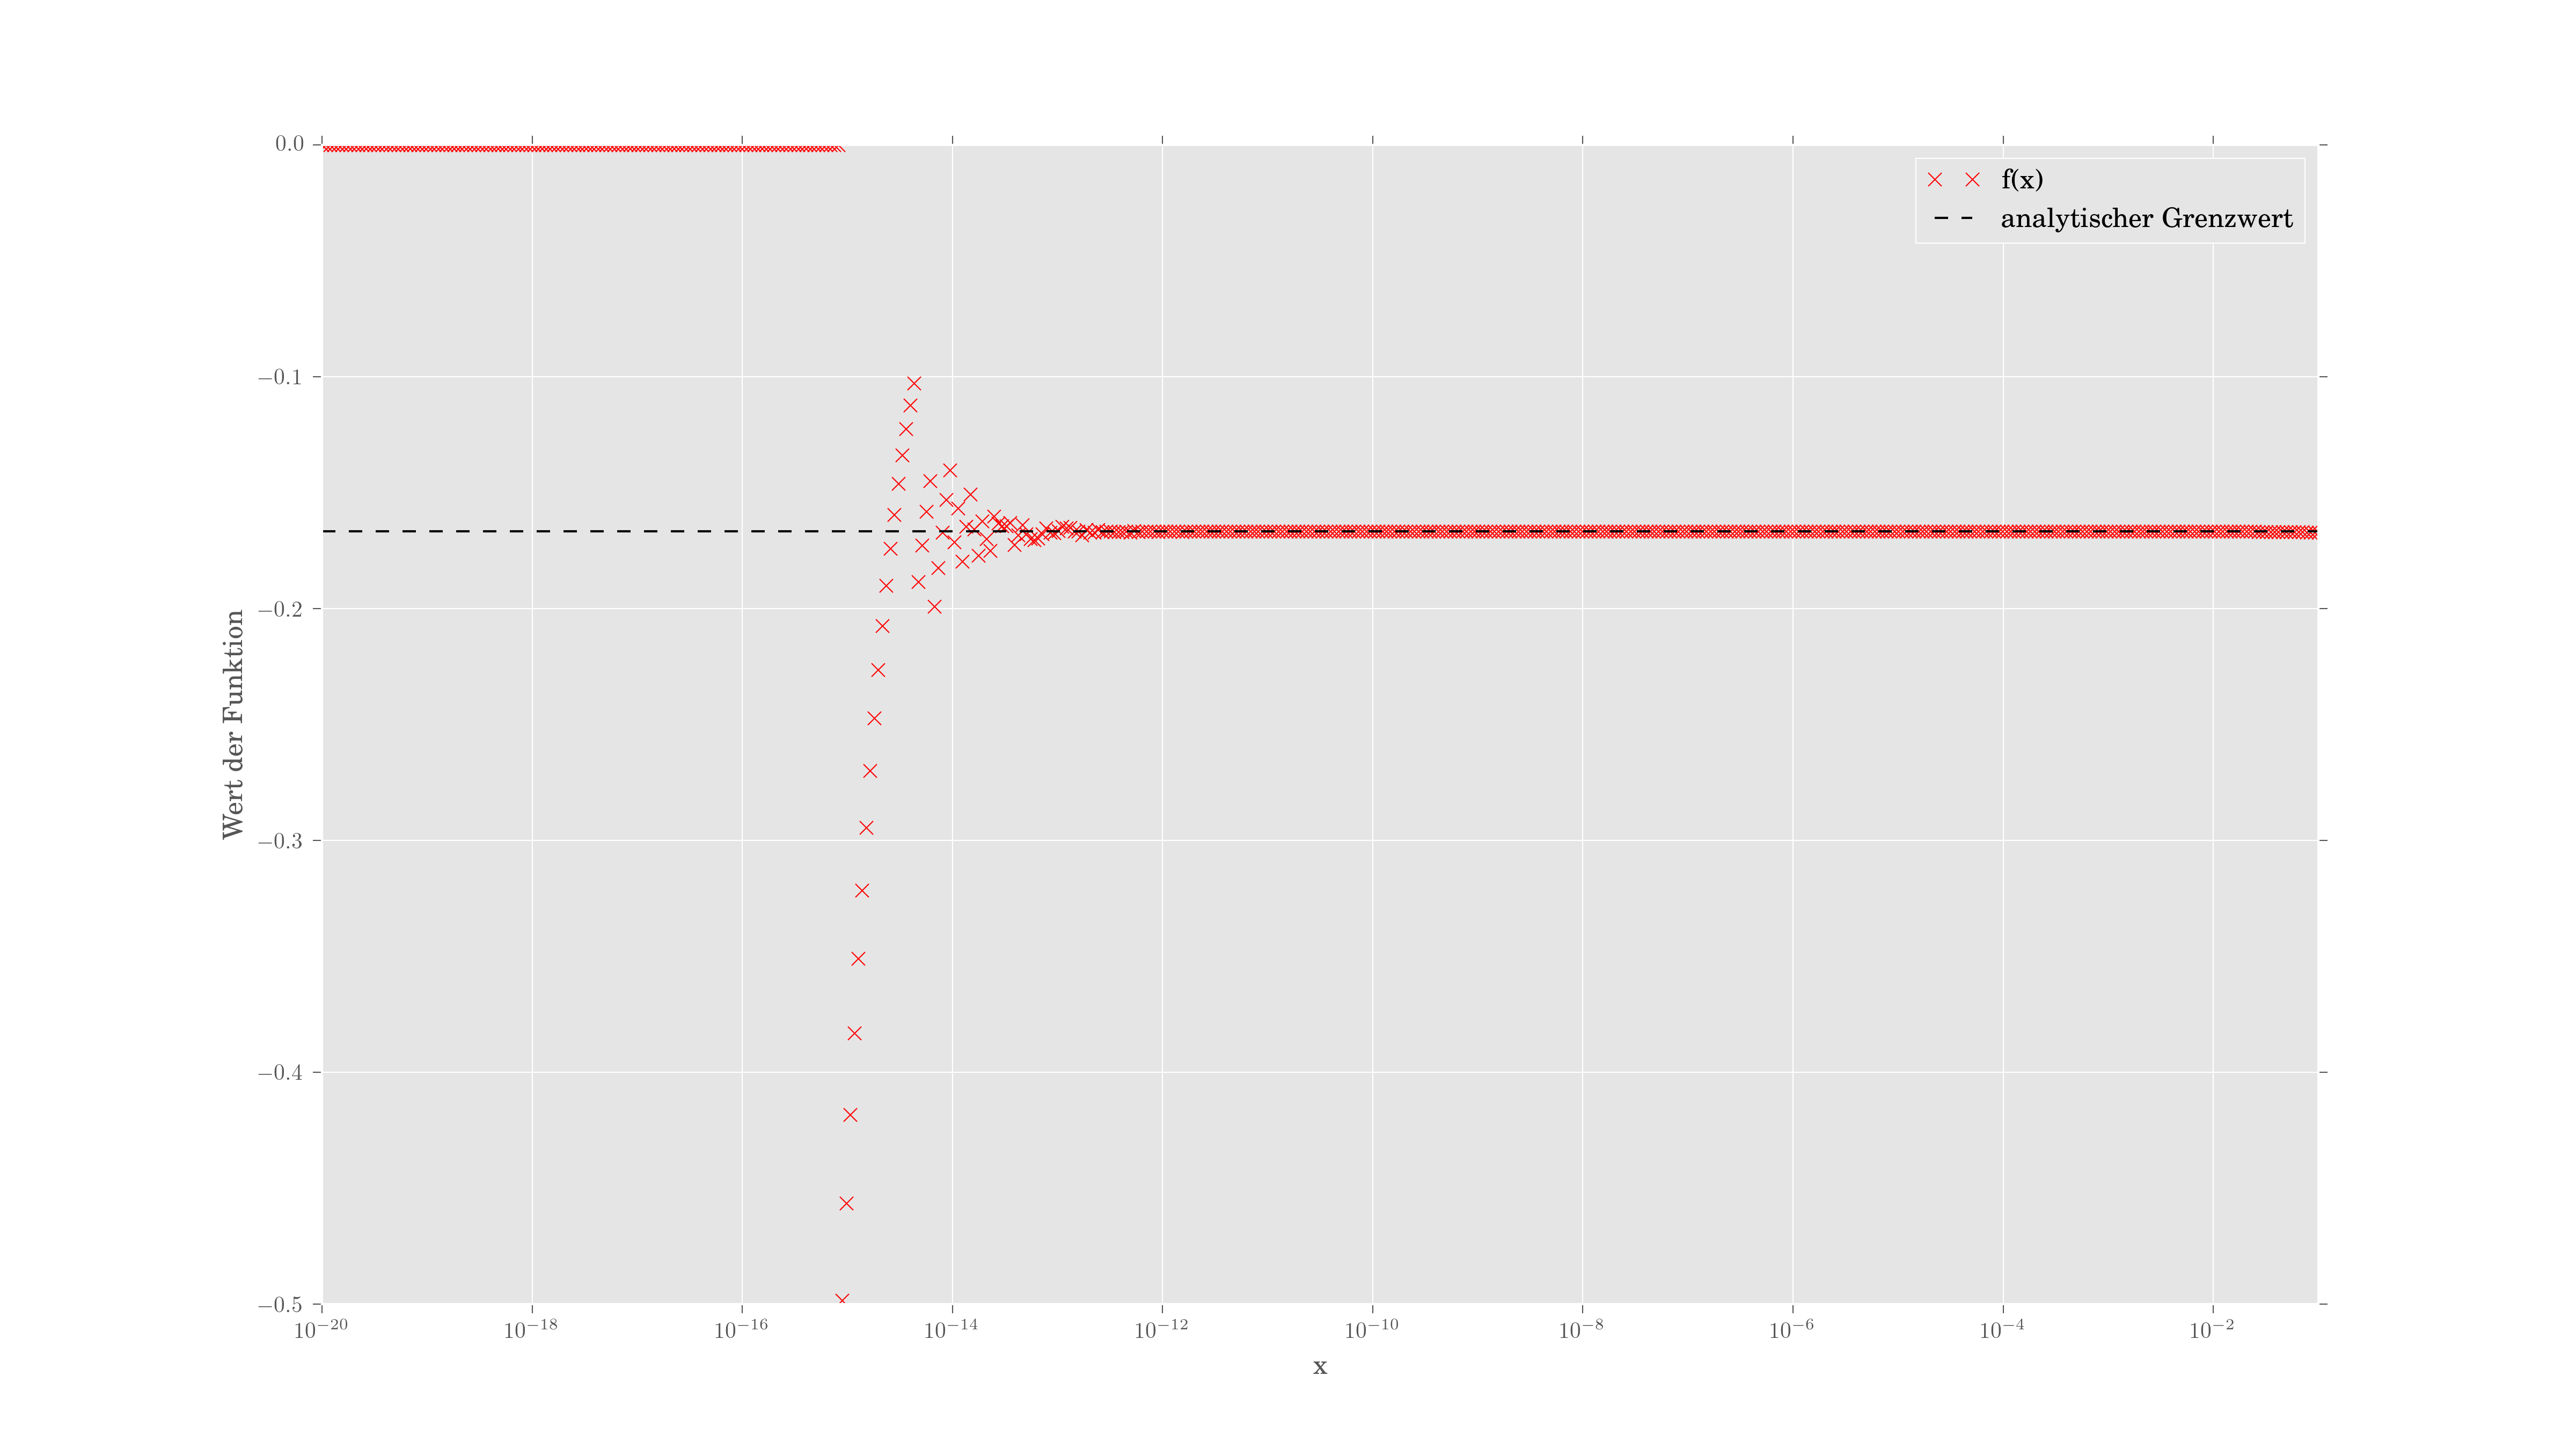
\includegraphics[width=\textwidth]{plot2.png}
\caption{Numerische Berechnug des Grenzwertes der gegebenen Funktion. Dazu wurden Werte von $0.1$ bis $10^{-20}$ eingesetzt und das Ergebnis grafisch dargestellt.}
\end{figure}
Die numerische Bestimmung des Grenzwertes scheitert für Werte von $x<10^{-13}$, da durch sehr kleine Zahlen dividiert wird.
\end{itemize}

\section{Aufgabe 3: \emph{Numerische Instabilität}}

Die Funktionen liefern für unterschiedliche Bereiche numerische Ergebnisse, die um nicht mehr als $1\%$ vom algebraischen Werte abweichen bzw. für die $f(x)=0$ oder $g(x)=0$ gilt.

\begin{itemize}

\item[a)] Für die Werte $10^{-20}\leq x \leq 1000$ weicht $f(x)$ nur um $1\%$ vom algebraischen Wert ab.\newline\newline
Für die Werte $1000000\leq x \leq 10^{20}$ gilt $f(x)=0$.

\item[b)] Für die Werte $0.0001\leq x \leq 10^{20}$ weicht $g(x)$ nur um $1\%$ vom algebraischen Wert ab.\newline\newline
Für die Werte $10^{-20} \leq x \leq 10^{-6}$ gilt $g(x)=0$.

\end{itemize}

\begin{figure}
\centering
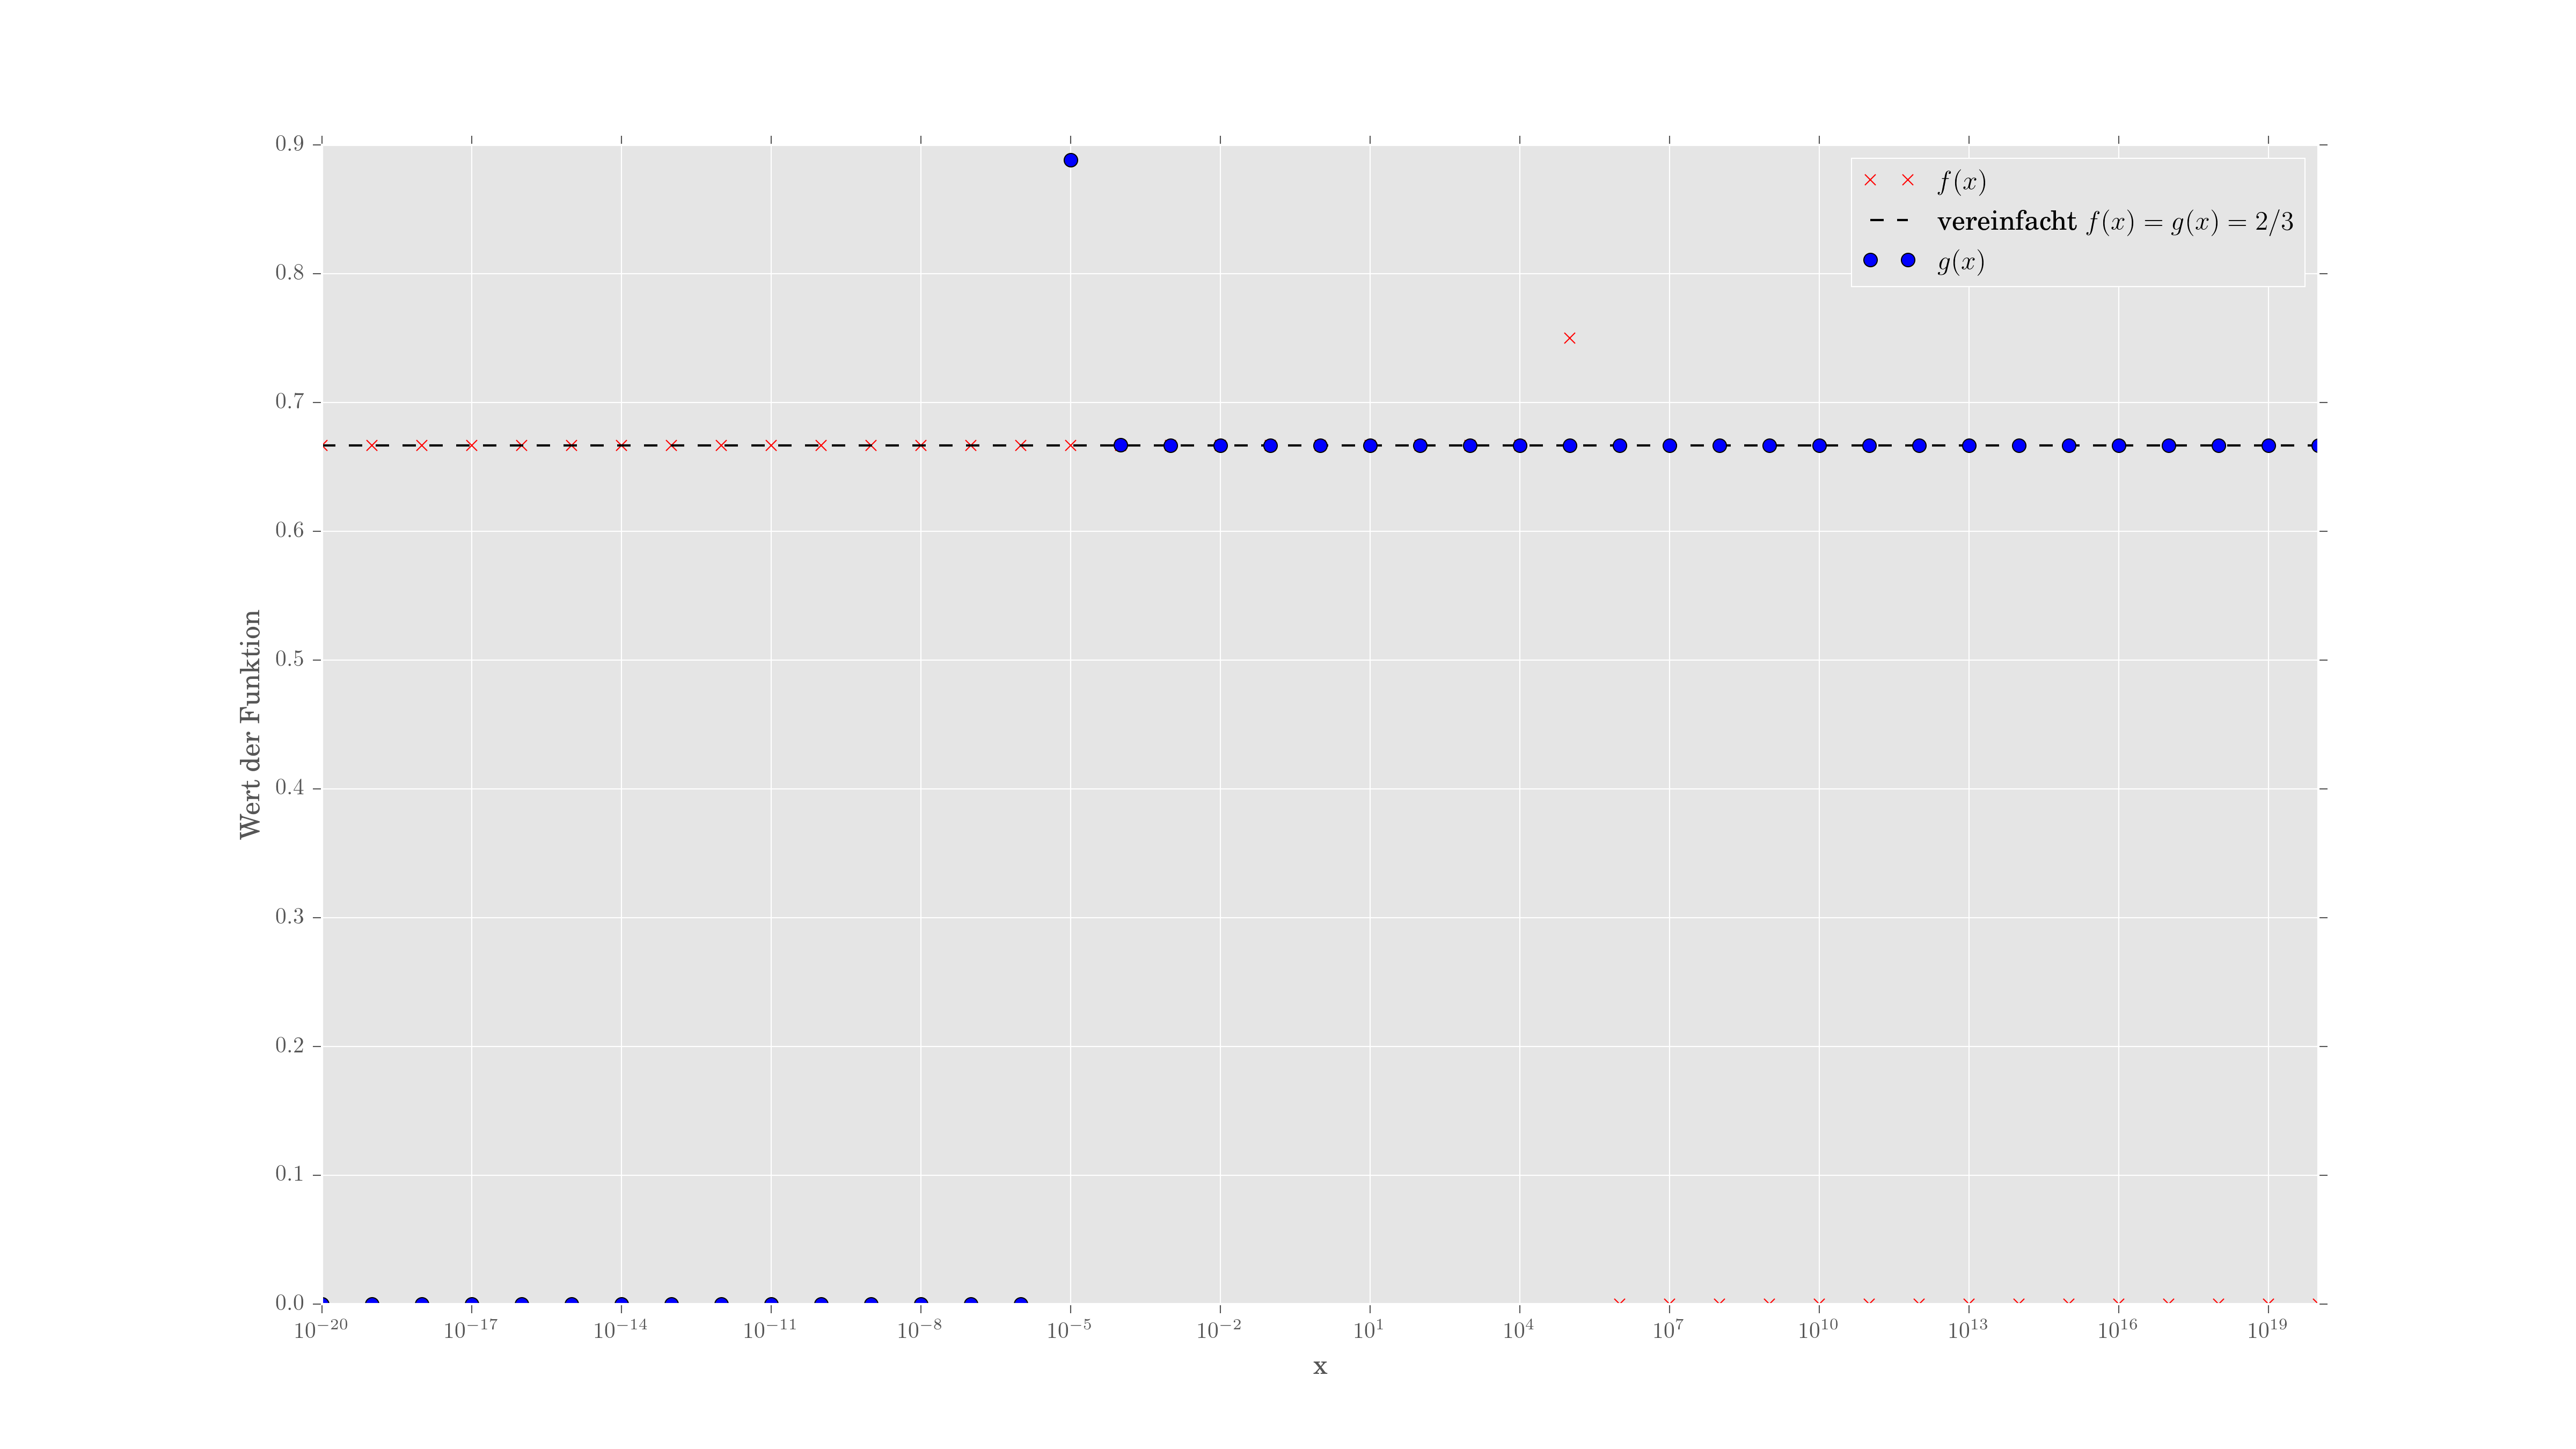
\includegraphics[width=\textwidth]{plot3.png}
\caption{Auswertung der Funktionen $g(x)$ und $f(x)$ im Vergleich mit dem analytischen Wert.}
\end{figure}

